\headline{{\textbf{\Large\sffamily TWBC Workshops:}}\\
          {\textbf{\large\sffamily Grafting the Paul's Scarlet Hawthorn}}}
\label{2025-02-hawthorn}
\noindent
The Common Hawthorn (\emph{Crataegus Monogyna}) is a beloved staple in the bonsai world, cherished for its robust character and delicate blossoms.
This versatile genus boasts over 200 species, each adorned with spiny branches, lobed leaves, and a knack for thriving in less\--than\--perfect conditions. 
Whether found along hedgerows or flourishing in neglected corners of gardens, the hawthorn's resilience makes it an excellent choice for both beginners and seasoned bonsai enthusiasts. 

Recognising a hawthorn in the wild is straightforward. 
Look for small, glossy leaves with distinctive lobes, clusters of white or pinkish flowers in spring, and bright red haws in autumn. 
The tree's spiny branches are not only a defining characteristic but also a natural deterrent to grazing animals, making it a survivor. 
For bonsai cultivation, hawthorns prefer a sunny spot and well\--draining soil. 
A light pruning in late winter encourages new growth, while regular fertilising ensures a healthy tree.

\medskip
\topic{Meet Paul's Scarlet}
\noindent
The Paul's Scarlet variety (\emph{Crataegus laevigata} `Paul's Scarlet') takes the charm of the hawthorn to an entirely new level. 
This cultivar dazzles with double, bright pink\--red flowers that form dense clusters, creating a truly vibrant spectacle in spring. 
Unlike its wild relatives, Paul's Scarlet is more ornamental and slightly less hardy. 
While standard hawthorns can shrug off the harshest conditions, Paul's Scarlet benefits from a touch more dedicated TLC.

Growing Paul's Scarlet as a bonsai requires attention to its slightly fussier nature. 
It's best kept protected from harsh winter winds, and regular checks for pests and diseases like mildew are essential. 
However, with care, this striking cultivar rewards its owner with a show\--stopping display that never fails to impress.

\begin{window}[%
    2,l,%
    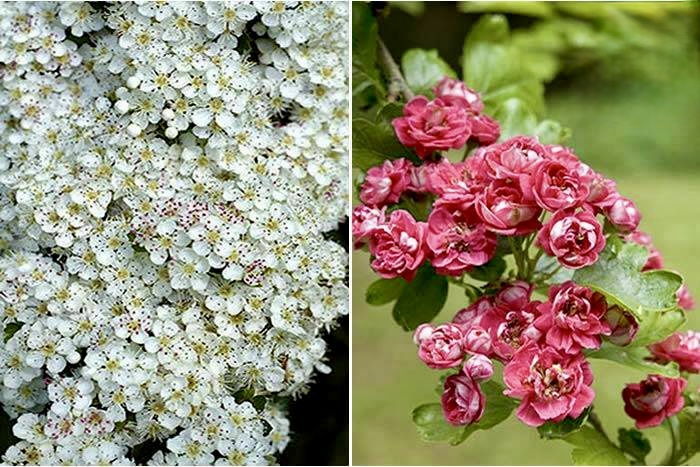
\includegraphics[width=1.0\columnwidth]{2025_02/res/hawthorn_comparison},%
    \centerline{\emph{Common Hawthorn \& Paul's Scarlet\---good choices for bonsai.}}%
]
\end{window}
\columnbreak

\topic{Grafting: Combining Strength and Beauty}
\noindent
Steve's workshop focuses on grafting Paul's Scarlet onto regular hawthorn rootstock, a technique that combines the best of both worlds. 
The hardy rootstock lends vigour and resilience, while the Paul's Scarlet scion provides its trademark floral splendour. 
Here's a quick summary of the process:

\begin{itemize}
	\item \textbf{Preparation:} Begin in late winter or early spring, when the rootstock is dormant. 
	Select a healthy hawthorn rootstock and a Paul's Scarlet scion with a similar branch diameter.
	
	\item \textbf{Making the Cuts:} Clean your tools thoroughly. 
	Make a slanted cut on both the scion and the rootstock, ensuring the cambium layers (the thin green layer beneath the bark) align perfectly.

	\item \textbf{Joining:} Fit the cuts together snugly and secure them with grafting tape. 
	This tight seal promotes healing and growth.
	
	\item \textbf{Sealing:} Apply grafting wax to protect the join from drying out and to deter pests.
\end{itemize}

\medskip
\topic{Aftercare for Your Grafted Bonsai}
\noindent
Your newly grafted bonsai will need some post\--operative pampering. 
Keep it in a sheltered spot, away from strong winds and direct sunlight, while the graft heals. 
Regular watering is crucial, but avoid water\-logging. 
As new growth appears, remove any shoots from the rootstock to direct energy into the grafted section.

With patience and dedication, your Paul's Scarlet hawthorn will flourish into a unique and vibrant bonsai specimen. 
Happy grafting, and may your trees thrive!
\closearticle
\vfill
\begin{center}
	
\includegraphics[width=0.9\columnwidth]{res/filler_b.png}
\end{center}
\columnbreak

